%% Charlie Redmon
%% 20170914
%% SEM path diagram

% standalone class for individual image to be included in a document
% border=15pt controls the whitespace padding around the diagram
\documentclass[border=15pt]{standalone}

% load custom style configurations from separate file
%% ------------------------------------------------------------
%% Charlie Redmon
%% 20170923
%% semTikzStyle.tex: style configurations for SEM path diagrams
%% ------------------------------------------------------------

\usepackage{tikz}

% observed variable
\tikzstyle{ov}=[shape=rectangle,
                draw=black!80,
                minimum height=0.6cm,
                minimum width=0.6cm,
                thick]

% response variable
\tikzstyle{av}=[shape=rectangle,
                draw=black!80,
                fill=black!10,
                minimum height=0.6cm,
                minimum width=0.6cm,
                thick]

% latent variable
\tikzstyle{lv}=[shape=circle,
                draw=black!80,
                thick,
                minimum width=1cm]

% correlations
\tikzstyle{lcor}=[bend left=30, dashed]
\tikzstyle{rcor}=[bend right=30, dashed]

% self-loops (for variance)
\tikzstyle{lloop}=[loop left, 
                   out=210, 
                   in=150, 
                   distance=0.3cm,
                   densely dotted]

\tikzstyle{rloop}=[loop right, 
                   out=30, 
                   in=-30, 
                   distance=0.3cm,
                   densely dotted]

\tikzstyle{aloop}=[loop above, 
                   out=60, 
                   in=120, 
                   distance=0.3cm,
                   densely dotted]

\tikzstyle{bloop}=[loop below, 
                   out=-60, 
                   in=-120, 
                   distance=0.3cm,
                   densely dotted]




\begin{document}

%% ">=stealth" sets the arrow head style
%% "semithick" sets the line width (0.6 pt)
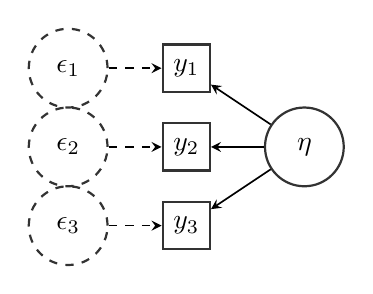
\begin{tikzpicture}[>=stealth,semithick]

% response variables
\node[ov] (y1) at (0,-1)      {$y_1$};
\node[ov] (y2) [below of=y1]  {$y_2$};
\node[ov] (y3) [below of=y2]  {$y_3$};

% error terms
\node[lv,dashed] (e1) at (-1.5, -1) {$\epsilon_1$};
\node[lv,dashed] (e2) at (-1.5, -2) {$\epsilon_2$};
\node[lv,dashed] (e3) at (-1.5, -3) {$\epsilon_3$};

% latent variable
\node[lv] (f1) at (1.5, -2)  {$\eta$};

% paths
\path[->] (f1) edge node[above,scale=0.6] {} (y1)
          (f1) edge node[above,scale=0.6] {} (y2)
          (f1) edge node[above,scale=0.6] {} (y3);
\path[->,dashed] (e1) edge node[above,scale=0.6] {} (y1)
          (e2) edge node[above,scale=0.6] {} (y2)
          (e3) edge node[above,scale=0.6] {} (y3);
\end{tikzpicture}


\end{document}